% Source: https://www.dropbox.com/sh/rl0yyth9g06psva/AADB0Cj4isIX5DAyrspqj8mFa
% File: "CS305 activity 12 binary search trees.pdf"
% Access: 05-18-2022

% comment out for student version
% \ifdefined\Student\relax\else\def\Teacher{}\fi

\documentclass[12pt]{article}

\title{Activity \#8: Binary Search Trees}
\author{Tammy VanDeGrift}
\newcommand{\activityeditor}{Preston Carman}
\newcommand{\activitysource}{\url{https://www.dropbox.com/sh/rl0yyth9g06psva/AADB0Cj4isIX5DAyrspqj8mFa}}
\date{Spring 2022}

\input{../../cspogil.sty}

% Included for drawing trees
\usepackage{tikz-qtree}
\usepackage{amssymb}
\tikzset{every tree node/.style={minimum width=2em,draw,circle},
         blank/.style={draw=none},
         edge from parent/.style=
         {draw,edge from parent path={(\tikzparentnode) -- (\tikzchildnode)}},
         level distance=1.25cm}

\begin{document}

  \begin{center}
    \maketitle
    \rolenames
  \end{center}

  Record your team's answers to the key questions (marked with key) below. \key
  \begin{enumerate}[label=(\alph*)]
    \itemsep 1.25in
    \item Model 2, Question \#7, 8
    \item Model 2, Question \#10
    \item Model 2, Question \#13
    \item Model 3, Question \#17
  \end{enumerate}

  \newpage
  \maketitle

  Binary search trees allow binary search for fast lookup, addition, and removal of data items, and can be used to implement dynamic sets and lookup tables.
  Since the nodes in a BST are laid out in such a way that each comparison skips about half of the remaining tree, the lookup performance is proportional to that of binary logarithm.

  \guide{
    \item Explain a binary search tree (BST)
    \item Knowledge of the rules for a BST
  }{
    \item Write code that adds and accesses a BST
  }{
    No additional notes.
  }

  \model{BST Basics}

  \quest{20 min}

  A \textbf{BINARY SEARCH} tree is a binary tree in which the data (keys) are stored in order such that all nodes to the right of node N have keys bigger than N and all nodes to the left of node N have keys smaller than N.

  \par\vskip 10pt

  BSTs give us a good data structure to implement the dictionary ADT (insert, find, delete, create, print).

  \par\vskip 10pt

  Here is a simple BST where the keys are ints:

  \par\vskip 10pt

  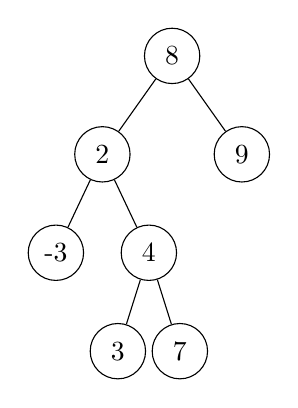
\begin{tikzpicture}
    \Tree
    [.8
    [.2
    -3
    [.4
    3
    7
    ]
    ]
    9
    ]
  \end{tikzpicture}

    \begin{itemize}
      \item Choose any node in the tree.
      \item Its left subtree descendants are less than the node's value.
      \item Its right subtree descendants are greater than the node's value.
    \end{itemize}

  \Q Is this a valid binary search tree? \ans[.3in]{\checkmark} yes \ans[.3in]{} no
    If no, explain why.
    \begin{answer}[1in]
      Yes, this is valid. All nodes in left subtree of each node are less than that node, and all nodes in right subtree are greater. Node 3 is the right child of 1 (3 > 1 ✓), and the entire subtree under 4 has values less than 5 (1,3 < 4 < 5 ✓).
    \end{answer}\par\vskip 5pt
    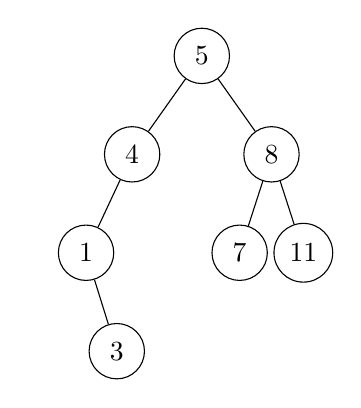
\begin{tikzpicture}
      \Tree
      [.5
              [.4
                      [.1
                          \edge[blank]; \node[blank]{};
                          3
                      ]
                  \edge[blank]; \node[blank]{};
              ]
              [.8
                  7
                  11
              ]
      ]
    \end{tikzpicture}

  \newpage

  \Q Is this a valid binary search tree? \ans[.3in]{} yes \ans[.3in]{\checkmark} no
    If no, explain why.
    \begin{answer}[1in]
      No, node 15 is in the right subtree of node 10, but 15 > 10, so 15 should be a right child. However, 10 is in the left subtree of 11, so all descendants of 10 must be less than 11. Since 15 > 11, this violates the BST property.
    \end{answer}\par\vskip 5pt
    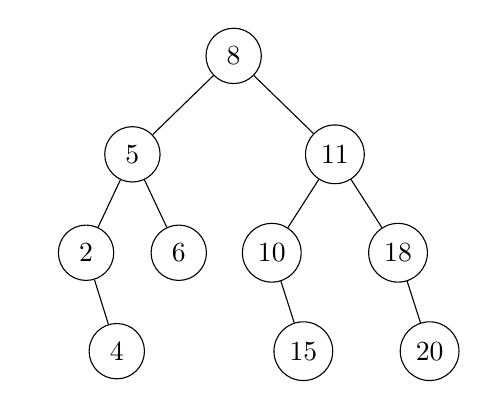
\begin{tikzpicture}
      \Tree
      [.8
              [.5
                      [.2
                          \edge[blank]; \node[blank]{};
                          4
                      ]
                  6
              ]
              [.11
                      [.10
                          \edge[blank]; \node[blank]{};
                          15
                      ]
                      [.18
                          \edge[blank]; \node[blank]{};
                          20
                      ]
              ]
      ]
    \end{tikzpicture}

  \Q Is this a valid binary search tree? \ans[.3in]{} yes \ans[.3in]{\checkmark} no
    If no, explain why.
    \begin{answer}[1in]
      No, node 6 is the right child of node 7, but 6 < 7. Right children must be greater than their parent, so this violates the BST property.
    \end{answer}\par\vskip 5pt
    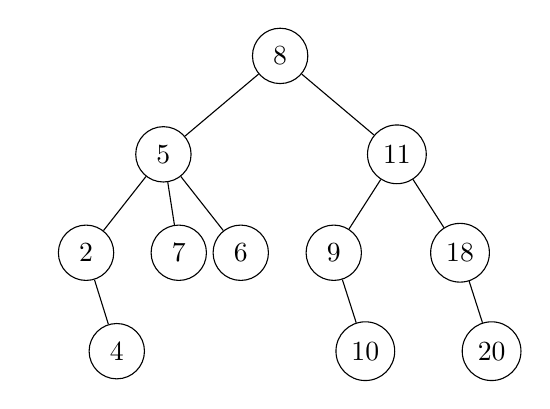
\begin{tikzpicture}
      \Tree
      [.8
              [.5
                      [.2
                          \edge[blank]; \node[blank]{};
                          4
                      ]
                  7
                  6
              ]
              [.11
                      [.9
                          \edge[blank]; \node[blank]{};
                          10
                      ]
                      [.18
                          \edge[blank]; \node[blank]{};
                          20
                      ]
              ]
      ]
    \end{tikzpicture}

  \textbf{Inserting new nodes}

  How do we insert new nodes into a BST?\par\vskip 5pt

  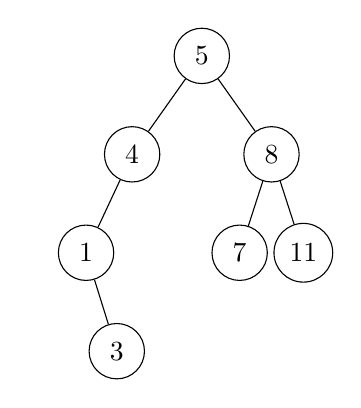
\begin{tikzpicture}
    \Tree
    [.5
            [.4
                    [.1
                        \edge[blank]; \node[blank]{};
                        3
                    ]
                \edge[blank]; \node[blank]{};
            ]
            [.8
                7
                11
            ]
    ]
  \end{tikzpicture}

  \Q Suppose we want to insert the value 6. Where does it go?
    \begin{answer}[1in]
      6 becomes the left child of 7 (6 > 5, go right; 6 < 8, go left; 6 < 7, go left; 7 has no left child, insert there).
    \end{answer}

  \Q Now, we want to insert 0. Where does it go?
    \begin{answer}[1in]
      0 becomes the left child of 1 (0 < 5, go left; 0 < 4, go left; 0 < 1, go left; 1 has no left child, insert there).
    \end{answer}

  \Q Now, we want to insert 9. Where does it go?
    \begin{answer}[1in]
      9 becomes the left child of 11 (9 > 5, go right; 9 > 8, go right; 9 < 11, go left; 11 has no left child, insert there).
    \end{answer}\par\vskip 5pt

  Inserting into a BST is quite simple. Insertions happen at the leaves.
  Here is an iterative version:
  \footnotesize
  \begin{cpplst}
/* insert
 * inserts data item d into tree; note that this is a BST so it is ordered
 */
void insert(TreeData d, TreeNode **tptr) {
    // create new node for data
    TreeNode *toInsert = newTreeNode(d);
    TreeNode *curr = *tptr;
    if (curr == NULL) {
        *tptr = toInsert; // make this the tree
        return;
    }
    // check value of t to see if new node should be to the right or left of curr
    while (curr != NULL) {
        if (d < curr->value) { // goes to left
            if (curr->left == NULL) {
                curr->left = toInsert;
                return;
            }
            // keep going left
            curr = curr->left;
        } else { // goes to right
            if (curr->right == NULL) {
                curr->right = toInsert;
                return;
            }
            // keep going right
            curr = curr->right;
        }
    }
}
/* newTreeNode
 * helper function, creates a new tree node with value d
 * returns the address of the new node
 */
TreeNode *newTreeNode(TreeData d) {
    TreeNode *toReturn = (TreeNode *)malloc(sizeof(TreeNode));
    toReturn->value = d;
    toReturn->left = NULL;
    toReturn->right = NULL;
    return toReturn;
}
  \end{cpplst}

  \normalsize

  Here is a recursive version to insert an item:

  \footnotesize
  \begin{cpplst}
/* insertR (this function is written recursively)
 * inserts data item d into tree; note that this is a BST so it is ordered
 */
void insertR(TreeData d, TreeNode **tptr) {
    if (*tptr == NULL) {
        *tptr = newTreeNode(d);
    } else if (d < (*tptr)->value) {
        insertR(d, &(*tptr)->left);
    } else {
        insertR(d, &(*tptr)->right);
    }
}
  \end{cpplst}
  \normalsize
  \newpage
  \model{Delete Node}

  \quest{10 min}

  The final dictionary operation that we need to examine is delete. Given the tree below, how would you delete each of the nodes (assume the deletions are independent, so you are starting with the same tree prior to each deletion).

  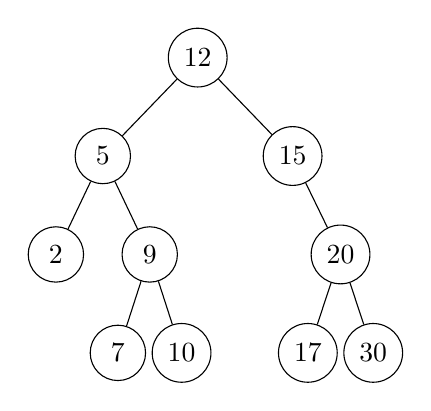
\begin{tikzpicture}
    \Tree
    [.12
    [.5
    2
        [.9
            7
            10
        ]
    ]
    [.15
    \edge[blank]; \node[blank]{};
    [.20
    17
    30
    ]
    ]
    ]
  \end{tikzpicture}

  \vskip -10pt

  \Q How would you delete 7?\key\\[-2.5mm]
    \begin{answer}[1in]
      7 is a leaf node. Simply delete it and set its parent (9) to have NULL as its left child.
    \end{answer}

  \vskip -10pt

  \Q How would you delete 15?\key\\[-2.5mm]
    \begin{answer}[1in]
      15 is an interior node with only a right child (20). Delete 15 and update its parent (12) to point to 15's right child (20).
    \end{answer}

  \Q How would you delete 5?
    \begin{answer}[1in]
      5 is an interior node with two children. Find successor: go right to 9, then left to 7 (leftmost). Copy 7's value to node 5. Delete leaf node 7.
    \end{answer}

  In general, here is the strategy for deletion:

  \par\vskip 10pt

  \textbf{Delete(D, T):}

  If Find(D, T) is false, do nothing.

  If T is a leaf node, delete it and update its parent to point to null instead of T.

  If T is an interior node and T has just a right child, delete T and update its parent to point to T's right child.

  If T is an interior node and T has just a left child, delete T and update its parent to point to T's left child.

  Else (T is interior with 2 children):

  \par\vskip 10pt

  Find the next successor of T by traversing to T's right child and then going all the way to the leftmost leaf.
  This leftmost leaf is the next largest item in the tree.
  Copy the value of this leftmost leaf to T.
  If leftmost leaf does not have a right subtree, delete leftmost leaf with same procedure as leaf node above.
  If leftmost leaf has a right subtree, then delete with the same procedure as interior node with just a right child.
  
  \vskip -10pt

  \Q Delete node 5 with procedure above. Cross out nodes that are deleted and values\key\\[-2.5mm] that are updated.
    \begin{answer}[1in]
      Node 5 has two children. Go right to 9, then left to 7 (successor). Copy 7 to node 5. Delete leaf 7. Result: node 5 becomes node 7, and the 7 leaf is removed.
    \end{answer}\par\vskip 5pt

    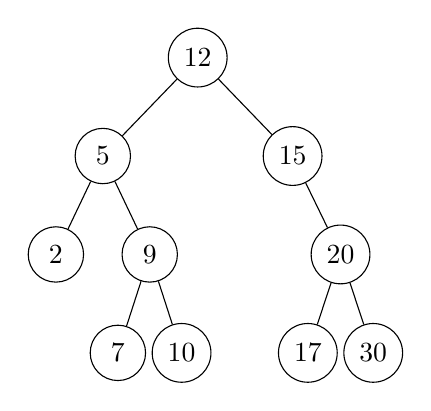
\begin{tikzpicture}
      \Tree
      [.12
      [.5
      2
          [.9
              7
              10
          ]
      ]
      [.15
      \edge[blank]; \node[blank]{};
      [.20
      17
      30
      ]
      ]
      ]
    \end{tikzpicture}

  \Q Delete node 10 with procedure above.
    Cross out nodes that are deleted and values that are updated.
    \begin{answer}[0.7in]
      Node 10 is a leaf. Simply delete it and set its parent (9) to have NULL as its right child.
    \end{answer}\par\vskip 5pt

    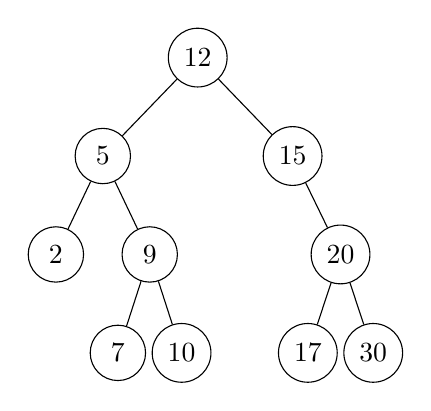
\begin{tikzpicture}
      \Tree
      [.12
      [.5
      2
          [.9
              7
              10
          ]
      ]
      [.15
      \edge[blank]; \node[blank]{};
      [.20
      17
      30
      ]
      ]
      ]
    \end{tikzpicture}

  \Q Delete node 15 with procedure above.
    Cross out nodes that are deleted and values that are updated.
    \begin{answer}[1in]
      Node 15 has only a right child (20). Delete 15 and update its parent (12) to point to 20 as its right child.
    \end{answer}\par\vskip 5pt

    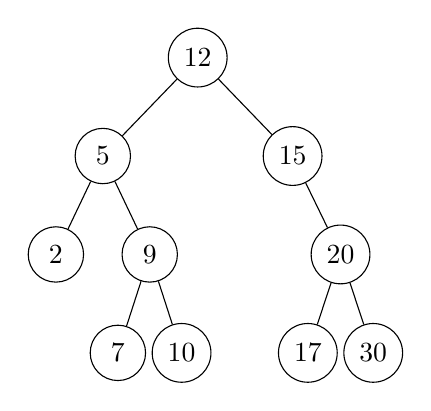
\begin{tikzpicture}
      \Tree
      [.12
      [.5
      2
          [.9
              7
              10
          ]
      ]
      [.15
      \edge[blank]; \node[blank]{};
      [.20
      17
      30
      ]
      ]
      ]
    \end{tikzpicture}\par\vskip 5pt

  Even though we are modeling BSTs with nodes having just one value, a (key, value) pair could be stored at each node, with the keys used as the comparison values when inserting, finding, and deleting.

  \Q Does your group have any questions about binary search trees?\key\\[-2.5mm]
    \begin{answer}[1in]
      Answers will vary
    \end{answer}
  \newpage
  \model{Creating a Tree}

  \quest{20 min}

  \textbf{Finding keys}

  Now, how would we find an element in the tree?\par\vskip 5pt

  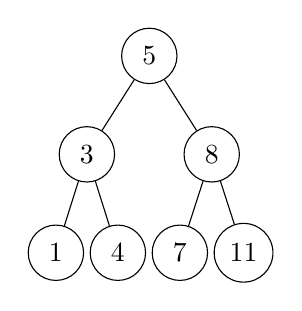
\begin{tikzpicture}
    \Tree
    [.5
            [.3
                1
                4
            ]
            [.8
                7
                11
            ]
    ]
  \end{tikzpicture}

  Let's find 7.
  Start with the root.
  If the item is equal to 7, return true (or a pointer to this item).
  If the item you are looking for is \textgreater ~ than the root, treat right subtree as root.
  Otherwise, treat left subtree as root.
  Keep applying this procedure until you hit a leaf.

  \Q What nodes are examined when looking for 7?
    \begin{answer}[0.5in]
      5, 8, 7
    \end{answer}

  \Q Now, look for 4. What nodes are examined when looking for 4?
    \begin{answer}[0.5in]
      5, 3, 4
    \end{answer}

  \par\vskip 10pt

  You will implement the find function in lab.

  \par\vskip 10pt

  \textbf{Creating a new tree}

  \par\vskip 10pt

  Creating a new tree is pretty straightforward.
  A tree with no items is NULL.

  \begin{cpplst}
    TreeNode * tree = NULL;
  \end{cpplst}

  To instantiate a tree with a list of items, we could do this:

  \begin{cpplst}
/* createTree
 * creates a binary search tree with data stored in array a
 */
TreeNode *createTree(TreeData a[], int size) {
    if (size <= 0) {
        return NULL;
    }
    TreeNode *toReturn = newTreeNode(a[0]); // insert first item from list
    int i;
    for (i = 1; i < size; i++) {
        insert(a[i], &toReturn);
    }
    return toReturn;
}
  \end{cpplst}

  An optional dictionary operation is size. Here is an implementation of size:

  \begin{cpplst}
/* size
 * returns the number of nodes in the tree
 */
int size(TreeNode *t) {
    if (t == NULL) {
        return 0;
    }
    return 1 + size(t->left) + size(t->right);
}
  \end{cpplst}

  Suppose you create an empty tree and items are inserted as follows:

  \begin{cpplst}
    TreeNode * tree = NULL;
    insert(5, &tree);
    insert(8, &tree);
    insert(2, &tree);
    insert(1, &tree);
    insert(10, &tree);
    insert(7, &tree);
    insert(9, &tree);
    insert(12, &tree);
  \end{cpplst}

  \Q What does the BST look like?
    \begin{answer}[2in]
      Root is 5. Left subtree: 2 (left of 5) with 1 as left child. Right subtree: 8 (right of 5) with left child 7 (which has right child 9) and right child 10 (which has right child 12).
    \end{answer}\par\vskip -10pt

  \Q What nodes are examined when finding 7?\key\\[-2.5mm]
    \begin{answer}[0.5in]
      5, 8, 7
    \end{answer}

  \Q What nodes are examined when finding 3?
    \begin{answer}[0.5in]
      5, 2 (then 3 is not found, would go right of 2 but NULL)
    \end{answer}

  \Q Now, suppose this is a new tree and insertions are done in this order:
    \begin{cpplst}
    TreeNode * tree = NULL;
    insert(1, &tree);
    insert(3, &tree);
    insert(4, &tree);
    insert(6, &tree);
    insert(7, &tree);
    insert(8, &tree);
    insert(9, &tree);
    \end{cpplst}

    What does this tree look like?
    \begin{answer}[2in]
      A completely skewed tree (linear chain). Root is 1, with only right children: 1->3->4->6->7->8->9. This is the worst case for BST, giving O(N) search time instead of O(log N).
    \end{answer}

  There are ways to balance trees, so we get the win of searches happening closer to $O(log_2N)$ rather than $O(N)$.
  You can read about specific kinds of trees, such as red-black trees and AVL trees that support tree rotations.

  \Q Give an insertion order of the same nodes in problem 4 that results in a full (complete) BST where most interior nodes have two children.
    Show the tree that results from this insertion order.
    \begin{answer}[2in]
      Insert in this order: 6, 3, 8, 1, 4, 7, 9. Root is 6, left subtree has 3 (with children 1 and 4), right subtree has 8 (with children 7 and 9). Height is 3, well-balanced.
    \end{answer}

\end{document}